% Created 2018-07-02 Mon 17:12
% Intended LaTeX compiler: pdflatex
\documentclass[10pt, compress, aspectratio=169, xcolor={table,usenames,dvipsnames}]{beamer}

\mode<beamer>{\usetheme[numbering=fraction, progressbar=none, titleformat=smallcaps, sectionpage=none]{metropolis}}
\input{beamer_configuration.tex}
\usetheme{default}
\author{\footnotesize Pedro Bruel \newline \scriptsize \emph{phrb@ime.usp.br}}
\date{\scriptsize \today}
\title{Autotuning: A Design of Experiments Approach}
\hypersetup{
 pdfauthor={\footnotesize Pedro Bruel \newline \scriptsize \emph{phrb@ime.usp.br}},
 pdftitle={Autotuning: A Design of Experiments Approach},
 pdfkeywords={},
 pdfsubject={},
 pdfcreator={Emacs 26.1 (Org mode 9.1.13)},
 pdflang={English}}
\begin{document}

\maketitle

\section{Autotuning}
\label{sec:orgaad0ce6}
\begin{frame}[fragile,label={sec:orgccfd287}]{Autotuning: Optimizing Program Configurations}
 \begin{columns}
\begin{column}{0.5\columnwidth}
\begin{block}{Architectures for High Performance Computing}
\begin{center}
\includegraphics[width=.9\linewidth]{../img/architectures.png}
\end{center}

How to write \alert{efficient code} for each of these?

\begin{block}{Autotuning}
\vspace{.2cm}

The process of \alert{automatically finding} a \alert{configuration} of a program that
optimizes an \alert{objective}
\end{block}
\end{block}
\end{column}

\begin{column}{0.5\columnwidth}
\begin{block}{Configurations}
\begin{itemize}
\item Program Configuration
\begin{itemize}
\item Algorithm, block size, \(\dots\)
\end{itemize}
\item \colorbox{Accent!25}{Source code transformation}
\begin{itemize}
\item Loop unrolling, tiling, rotation \(\dots\)
\end{itemize}
\item Compiler configuration
\begin{itemize}
\item \texttt{-O2}, vectorization, \(\dots\)
\end{itemize}
\item \(\dots\)
\end{itemize}

\begin{block}{Objectives}
\begin{itemize}
\item \colorbox{Accent!25}{Execution time}
\item Memory \& power consumption
\item \(\dots\)
\end{itemize}
\end{block}
\end{block}
\end{column}
\end{columns}
\end{frame}

\begin{frame}[label={sec:org63ad28f}]{Autotuning: Search Spaces}
\begin{columns}
\begin{column}{0.4\columnwidth}
\begin{block}{Search Spaces}
\vspace{.2cm}

Represent the \alert{effect} of all possible
\alert{configurations} on the \alert{objectives}
\begin{block}{Issues}
\begin{itemize}
\item \alert{Exponential Growth}
\item \alert{Geometry}
\item \alert{Measurement Time}
\end{itemize}
\end{block}
\end{block}
\end{column}
\begin{column}{0.6\columnwidth}
\begin{center}
\begin{center}
\includegraphics[width=.9\linewidth]{../img/holder_table.pdf}
\end{center}

\alert{Hölder Table Function}
\end{center}
\end{column}
\end{columns}
\end{frame}

\begin{frame}[label={sec:orge7459d5}]{Autotuning: Multiple Approaches}
\begin{columns}
\begin{column}{0.5\columnwidth}
\begin{block}{Popular Approaches}
\footnotesize
\begin{itemize}
\item \colorbox{red!25}{Exhaustive}
\item \colorbox{green!25}{Meta-Heuristics}
\item \colorbox{cyan!25}{Machine Learning}
\end{itemize}
\normalsize

\vspace{-.4cm}

\begin{table}
    \centering
    \begin{tabular}{@{}lll@{}}
        \toprule
        System & Domain & Approach \\ \midrule
        \rowcolor{red!25} ATLAS & Dense Linear Algebra & Exhaustive\\ \addlinespace
        \rowcolor{green!25} INSIEME & Compiler & Genetic Algorithm \\
        \rowcolor{green!25} Active Harmony & Runtime & Nelder-Mead \\
        \rowcolor{green!25} ParamILS & Domain-Agnostic & Stochastic Local Search \\
        \rowcolor{green!25} OPAL & Domain-Agnostic & Direct Search \\
        \rowcolor{green!25} OpenTuner & Domain-Agnostic & Ensemble \\ \addlinespace
        \rowcolor{cyan!25} MILEPOST GCC & Compiler & Machine Learning \\
        \rowcolor{cyan!25} Apollo & GPU kernels & Decision Trees \\ \addlinespace
        \bottomrule
    \end{tabular}
\end{table}

\end{block}
\end{column}

\begin{column}{0.5\columnwidth}
\begin{block}{Main Issues}
\vspace{0.2cm}

These approaches \alert{assume}:

\begin{itemize}
\item A \alert{large number of function evaluations}
\item Seach space \alert{``smoothness''}
\item Good solutions are \alert{reachable}
\end{itemize}

After optimizing:

\begin{itemize}
\item \alert{Learn nothing} about the search space
\item \alert{Can't explain} why optimizations work
\end{itemize}
\end{block}
\end{column}
\end{columns}
\end{frame}
\section{Applying Design of Experiments to Autotuning}
\label{sec:orgba80df7}
\begin{frame}[label={sec:org9ce7fb3}]{Applying Design of Experiments to Autotuning}
\begin{columns}
\begin{column}{0.5\columnwidth}
\begin{block}{Our Approach}
\vspace{.2cm}

Using \alert{efficient experimental designs} to overcome issues
related to \alert{exponential growth}, \alert{geometry}, and
\alert{measurement time}

\begin{block}{Design Requirements}
\begin{itemize}
\item Support a large number of factors (\alert{Exponential Growth})
\item Support numerical and categorical factors (\alert{Geometry})
\item Minimize function evaluations (\alert{Measurement Time})
\end{itemize}
\end{block}
\end{block}
\end{column}

\begin{column}{0.5\columnwidth}
\begin{block}{Main Candidate: \alert{D-Optimal Designs}}
\vspace{.2cm}

\begin{itemize}
\item Require an \alert{initial model}
\item Minimize \alert{variance of estimators}
\item Support \alert{mixed-level factors}
\item Constructed using \alert{search algorithms}
\end{itemize}
\end{block}
\end{column}
\end{columns}
\end{frame}

\begin{frame}[fragile,label={sec:org74a9c18}]{D-Optimal Designs: Example in R}
 \begin{columns}
\begin{column}{0.5\columnwidth}
\begin{block}{Example}
\begin{itemize}
\item Factors \& Levels: \(\mathbf{X} = \{x_1 = \{1, 2, 3\}, x_2 = \{1, 2, 3\}\}\)
\item Model: \(\mathbf{Y} = \mathbf{X}\beta + \eta\)
\item Minimize: \alert{D-optimality}
\item Candidate set: \alert{Full factorial}
\item Construction method: \alert{Fedorov's algorithm}
\end{itemize}

\begin{block}{Source code}
\lstset{language=r,label= ,caption= ,captionpos=b,numbers=none}
\begin{lstlisting}
library(AlgDesign)
full_factorial <- gen.factorial(c(3, 3),
                      factors = c(1, 2))
output <- optFederov(~., full_factorial,
                     nTrials = 5)
\end{lstlisting}
\end{block}
\end{block}
\end{column}

\begin{column}{0.5\columnwidth}
\begin{block}{Output}
\scriptsize

\begin{verbatim}
$D
[1] 0.2

$A
[1] 13

$Ge
[1] 0.333

$Dea
[1] 0.135

$design
   2   3   6   7   9
X1 "2" "3" "3" "1" "3"
X2 "1" "1" "2" "3" "3"

$rows
[1] 2 3 6 7 9
\end{verbatim}

\normalsize
\end{block}
\end{column}
\end{columns}
\end{frame}
\section{Case Study: A Laplacian GPU Kernel}
\label{sec:orgb51c700}
\begin{frame}[label={sec:org6af4f4f}]{Case Study: A Laplacian GPU Kernel}
\begin{columns}
\begin{column}{0.5\columnwidth}
\begin{block}{Search Space}
\vspace{-.2cm}

\begin{table}[]
\footnotesize
\begin{tabular}{@{}m{0.39\columnwidth}m{0.35\columnwidth}@{}}
\toprule
Parameters & Values \\ \midrule
\textit{vector\_length} & 1, 2, 4, 8, 16 \\
\textit{load\_overlap} & true, false \\
\textit{temporary\_size} & 2, 4 \\
\textit{elements\_number} & 1 - 24 \\
\textit{y\_component\_number} & 1 - 6 \\
\textit{threads\_number} & 32, 64, 128, 256, 512, 1024 \\
\textit{lws\_y} & 1, 2, 4, 8, 16, 32, 64, 128, 256, 512, 1024 \\ \bottomrule
\end{tabular}
\end{table}

\end{block}
\end{column}
\begin{column}{0.5\columnwidth}
\begin{block}{Objective}
\vspace{.2cm}

Time to compute each pixel:
\begin{itemize}
\item \(\alert{time\_per\_pixel}\)
\end{itemize}

\begin{block}{Initial Model}
\scriptsize
\begin{align*}
      \alert{time\_per\_pixel} = & \; y\_component\_number + 1 / y\_component\_number + \\
                        & \; vector\_length + lws\_y + 1 / lws\_y + \\
                        & \; load\_overlap + temporary\_size + \\
                        & \; elements\_number + 1 / elements\_number + \\
                        & \; threads\_number + 1 / threads\_number
\end{align*}
\normalsize
\end{block}
\end{block}
\end{column}
\end{columns}
\end{frame}
\begin{frame}[label={sec:orgdeb0086}]{Strategy}
\begin{center}
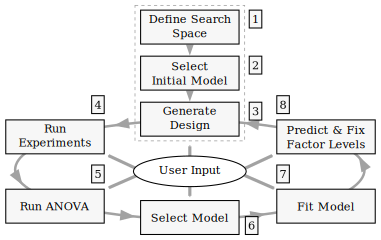
\includegraphics[width=0.63\textwidth]{../img/doe_anova_strategy.eps}
\end{center}
\end{frame}
\begin{frame}[fragile,label={sec:org6747ff6}]{Loading Data}
 \lstset{language=r,label= ,caption= ,captionpos=b,numbers=none}
\begin{lstlisting}
library(AlgDesign)
library(car)
library(dplyr)
\end{lstlisting}

\scriptsize

\lstset{language=r,label= ,caption= ,captionpos=b,numbers=none}
\begin{lstlisting}
complete_data = read.csv("../data/search_space.csv", header = TRUE)
str(complete_data)
\end{lstlisting}

\begin{verbatim}
'data.frame':	23120 obs. of  9 variables:
 $ elements_number   : int  3 2 4 2 2 2 2 4 4 3 ...
 $ y_component_number: int  3 2 1 1 1 2 2 2 4 1 ...
 $ vector_length     : int  4 1 4 1 8 2 1 8 16 4 ...
 $ temporary_size    : int  4 2 2 2 2 2 4 4 2 4 ...
 $ vector_recompute  : Factor w/ 1 level "true": 1 1 1 1 1 1 1 1 1 1 ...
 $ load_overlap      : Factor w/ 2 levels "false","true": 2 1 2 1 2 2 1 2 2 2 ...
 $ threads_number    : int  64 128 64 256 128 128 128 64 128 32 ...
 $ lws_y             : int  64 1 32 64 32 8 2 2 128 32 ...
 $ time_per_pixel    : num  1.11e-08 1.58e-10 2.34e-09 1.39e-09 3.40e-09 ...
\end{verbatim}

\normalsize
\end{frame}

\begin{frame}[fragile,label={sec:orgccad59c}]{Configuration}
 \lstset{language=r,label= ,caption= ,captionpos=b,numbers=none}
\begin{lstlisting}
used <- 0
budget <- 120

iterations <- 1

factors = c("elements_number", "y_component_number",
            "vector_length", "temporary_size",
            "load_overlap", "threads_number",
            "lws_y")

data <- complete_data[, c(factors, "time_per_pixel")]
\end{lstlisting}
\end{frame}

\begin{frame}[fragile,label={sec:orge77077e}]{Step 1: D-Optimal Design}
 \scriptsize
\lstset{language=r,label= ,caption= ,captionpos=b,numbers=none}
\begin{lstlisting}
output <- optFederov(~ y_component_number + I(1 / y_component_number) +
                       vector_length + lws_y + I(1 / lws_y) +
                       load_overlap + temporary_size +
                       elements_number + I(1 / elements_number) +
                       threads_number + I(1 / threads_number),
                     data,
                     nTrials = 24)

federov_design <- data[output$rows, ]
experiments <- output$rows

str(federov_design)
\end{lstlisting}

\begin{verbatim}
'data.frame':	24 obs. of  8 variables:
 $ elements_number   : int  1 4 2 3 1 4 24 24 12 8 ...
 $ y_component_number: int  1 1 2 3 1 1 6 6 3 2 ...
 $ vector_length     : int  16 1 1 16 1 1 16 16 1 16 ...
 $ temporary_size    : int  2 4 2 4 4 2 4 2 4 2 ...
 $ load_overlap      : Factor w/ 2 levels "false","true": 1 2 2 2 2 1 2 1 1 1 ...
 $ threads_number    : int  32 32 128 256 128 128 256 128 32 1024 ...
 $ lws_y             : int  32 1 1 32 1 64 32 1 1 16 ...
 $ time_per_pixel    : num  4.31e-08 3.47e-10 1.57e-10 3.53e-09 2.29e-10 ...
\end{verbatim}

\normalsize
\end{frame}

\begin{frame}[fragile,label={sec:org3e0c3f7}]{Step 1: Regression}
 \scriptsize
\lstset{language=r,label= ,caption= ,captionpos=b,numbers=none}
\begin{lstlisting}
regression <- lm(time_per_pixel ~ y_component_number + I(1 / y_component_number) +
                                  vector_length + lws_y + I(1 / lws_y) +
                                  load_overlap + temporary_size +
                                  elements_number + I(1 / elements_number) +
                                  threads_number + I(1 / threads_number),
                  data = federov_design)
summary.aov(regression)
\end{lstlisting}

\begin{verbatim}
                        Df    Sum Sq   Mean Sq F value  Pr(>F)
y_component_number       1 2.075e-16 2.075e-16   5.089 0.04353 *
I(1/y_component_number)  1 1.942e-16 1.942e-16   4.763 0.04968 *
vector_length            1 5.829e-16 5.829e-16  14.297 0.00262 **
lws_y                    1 3.824e-16 3.824e-16   9.379 0.00985 **
I(1/lws_y)               1 2.346e-16 2.346e-16   5.754 0.03360 *
load_overlap             1 1.125e-16 1.125e-16   2.759 0.12258
temporary_size           1 3.333e-16 3.333e-16   8.175 0.01438 *
elements_number          1 1.549e-16 1.549e-16   3.799 0.07503 .
I(1/elements_number)     1 3.013e-16 3.013e-16   7.389 0.01867 *
threads_number           1 4.329e-16 4.329e-16  10.618 0.00685 **
I(1/threads_number)      1 2.201e-16 2.201e-16   5.399 0.03851 *
Residuals               12 4.893e-16 4.080e-17
---
Signif. codes:  0 ‘***’ 0.001 ‘**’ 0.01 ‘*’ 0.05 ‘.’ 0.1 ‘ ’ 1
\end{verbatim}

\normalsize
\end{frame}

\begin{frame}[label={sec:orgc4f895c}]{Step 1: Heteroscedasticity}
\begin{center}
\includegraphics[width=0.7\textwidth]{../img/regression_before_transform.png}
\end{center}
\end{frame}

\begin{frame}[fragile,label={sec:orgefa5f29}]{Step 1: Power Transform}
 \lstset{language=r,label= ,caption= ,captionpos=b,numbers=none}
\begin{lstlisting}
boxcox_transform <- powerTransform(time_per_pixel ~ y_component_number +
                                      I(1 / y_component_number) +
                                      vector_length + lws_y + I(1 / lws_y) +
                                      load_overlap + temporary_size +
                                      elements_number + I(1 / elements_number) +
                                      threads_number + I(1 / threads_number),
                                   data = federov_design)

regression <- lm(bcPower(time_per_pixel, boxcox_transform$lambda) ~ y_component_number +
                                I(1 / y_component_number) +
                                vector_length + lws_y + I(1 / lws_y) +
                                load_overlap + temporary_size +
                                elements_number + I(1 / elements_number) +
                                threads_number + I(1 / threads_number),
                             data = federov_design)
\end{lstlisting}
\end{frame}

\begin{frame}[fragile,label={sec:orga309dce}]{Step 1: Power Transform Results}
 \scriptsize
\lstset{language=r,label= ,caption= ,captionpos=b,numbers=none}
\begin{lstlisting}
summary.aov(regression)
\end{lstlisting}

\begin{verbatim}
                        Df Sum Sq Mean Sq F value   Pr(>F)
y_component_number       1 0.0952  0.0952   6.284 0.027568 *
I(1/y_component_number)  1 0.0437  0.0437   2.886 0.115128
vector_length            1 0.7588  0.7588  50.088 1.29e-05 ***
lws_y                    1 0.5678  0.5678  37.477 5.16e-05 ***
I(1/lws_y)               1 0.2999  0.2999  19.797 0.000794 ***
load_overlap             1 0.0003  0.0003   0.022 0.885236
temporary_size           1 0.0389  0.0389   2.569 0.134980
elements_number          1 0.0662  0.0662   4.372 0.058475 .
I(1/elements_number)     1 0.0143  0.0143   0.945 0.350303
threads_number           1 0.3009  0.3009  19.860 0.000784 ***
I(1/threads_number)      1 0.1549  0.1549  10.224 0.007667 **
Residuals               12 0.1818  0.0152
---
Signif. codes:  0 ‘***’ 0.001 ‘**’ 0.01 ‘*’ 0.05 ‘.’ 0.1 ‘ ’ 1
\end{verbatim}

\normalsize
\end{frame}
\begin{frame}[label={sec:org076ecc9}]{Step 1: Power Transform Results}
\begin{center}
\includegraphics[width=0.7\textwidth]{../img/regression_after_transform.png}
\end{center}
\end{frame}
\begin{frame}[fragile,label={sec:org2a3434d}]{Step 1: Predicting Best Point and Pruning Data}
 \lstset{language=r,label= ,caption= ,captionpos=b,numbers=none}
\begin{lstlisting}
predicted_best <- data[predict(regression, data) == min(predict(regression, data)), ]
best <- complete_data[complete_data$time_per_pixel == min(complete_data$time_per_pixel), ]
best_row <- rownames(best)

predicted_best$slowdown <- predicted_best$time_per_pixel / best$time_per_pixel
predicted_best$method <- rep("DOPTaov_t", nrow(predicted_best))
predicted_best$point_number <- rep(used, nrow(predicted_best))
predicted_best$vector_recompute <- rep("true", nrow(predicted_best))

data <- complete_data[complete_data$vector_length == predicted_best$vector_length &
                      complete_data$lws_y == predicted_best$lws_y, c(factors, "time_per_pixel")]
scaled_data <- data[, factors]
\end{lstlisting}
\end{frame}
\begin{frame}[fragile,label={sec:org0977c97}]{Step 1: Predicting Best Point and Pruning Data}
 \scriptsize
\lstset{language=r,label= ,caption= ,captionpos=b,numbers=none}
\begin{lstlisting}
predicted_best
str(data)
\end{lstlisting}

\begin{verbatim}
     elements_number y_component_number vector_length temporary_size
9978              12                  3             1              4
     load_overlap threads_number lws_y time_per_pixel slowdown    method
9978        false           1024     1    2.33811e-10 2.006939 DOPTaov_t
     point_number vector_recompute
9978           24             true
'data.frame':	576 obs. of  8 variables:
 $ elements_number   : int  2 4 4 1 3 3 3 4 4 4 ...
 $ y_component_number: int  2 1 1 1 1 3 1 2 2 1 ...
 $ vector_length     : int  1 1 1 1 1 1 1 1 1 1 ...
 $ temporary_size    : int  2 4 2 4 4 2 2 4 4 4 ...
 $ load_overlap      : Factor w/ 2 levels "false","true": 1 1 1 1 1 1 2 1 2 1 ...
 $ threads_number    : int  128 64 128 256 256 128 512 64 64 512 ...
 $ lws_y             : int  1 1 1 1 1 1 1 1 1 1 ...
 $ time_per_pixel    : num  1.58e-10 3.03e-10 3.01e-10 2.36e-10 3.33e-10 ...
\end{verbatim}
\normalsize
\end{frame}
\begin{frame}[fragile,label={sec:org99a2ed0}]{Subsequent Steps}
 We can now \alert{continue} with the \alert{other steps}:
\scriptsize
\lstset{language=r,label= ,caption= ,captionpos=b,numbers=none}
\begin{lstlisting}
predicted_best
\end{lstlisting}

\begin{verbatim}
      elements_number y_component_number vector_length temporary_size
17258               6                  6             1              2
      vector_recompute load_overlap threads_number lws_y time_per_pixel
17258             true         true            256     1     1.1792e-10
      point_number    method slowdown
17258           56 DOPTaov_t 1.012177
\end{verbatim}

\normalsize
\end{frame}

\begin{frame}[label={sec:org51010a1}]{Comparing Strategies}
% latex table generated in R 3.4.4 by xtable 1.8-2 package
% Mon Jul  2 17:12:27 2018
\begin{table}[ht]
\centering
\begingroup\small
\begin{tabular}{lrrrrrrrr}
  \hline
 & Min. & 1st Qu. & Median & Mean & 3rd Qu. & Max. & Mean Pt. & Max Pt. \\
  \hline
RS & 1.00 & 1.03 & 1.08 & 1.10 & 1.18 & 1.39 & 120.00 & 125.00 \\
  LHS & 1.00 & 1.09 & 1.19 & 1.17 & 1.24 & 1.52 & 98.92 & 125.00 \\
  GS & 1.00 & 1.35 & 1.80 & 6.46 & 6.31 & 124.76 & 22.17 & 106.00 \\
  GSR & 1.00 & 1.07 & 1.19 & 1.23 & 1.33 & 3.16 & 120.00 & 120.00 \\
  GA & 1.00 & 1.02 & 1.09 & 1.12 & 1.19 & 1.65 & 120.00 & 120.00 \\
  LM & 1.01 & 1.01 & 1.01 & 1.02 & 1.01 & 3.77 & 119.00 & 119.00 \\
  LMB & 1.01 & 1.01 & 1.03 & 1.03 & 1.03 & 3.80 & 104.81 & 106.00 \\
  LMBT & 1.01 & 1.01 & 1.03 & 1.03 & 1.03 & 1.98 & 104.89 & 106.00 \\
  RQ & 1.01 & 1.01 & 1.01 & 1.02 & 1.01 & 2.06 & 119.00 & 119.00 \\
  DOPT & 1.38 & 1.64 & 1.64 & 1.68 & 1.64 & 2.91 & 120.00 & 120.00 \\
  DLM & 1.01 & 1.01 & 1.01 & 1.01 & 1.01 & 1.08 & 54.85 & 56.00 \\
  DLMT & 1.01 & 1.01 & 1.01 & 1.01 & 1.01 & 1.01 & 54.84 & 56.00 \\
   \hline
\end{tabular}
\endgroup
\caption{Summary statistics}
\end{table}
\end{frame}
\maketitle
\end{document}
